% IEEE standard conference template; to be used with:
%   spconf.sty  - LaTeX style file, and
%   IEEEbib.bst - IEEE bibliography style file.
% --------------------------------------------------------------------------

\documentclass[letterpaper]{article}
\usepackage{spconf,amsmath,amssymb,graphicx}

% Example definitions.
% --------------------
% nice symbols for real and complex numbers
\newcommand{\R}[0]{\mathbb{R}}
\newcommand{\C}[0]{\mathbb{C}}

% bold paragraph titles
\newcommand{\mypar}[1]{{\bf #1.}}

% Title.
% ------
\title{A Descriptive Title, not too general, not too long}
%
% Single address.
% ---------------
\name{Markus P\"uschel\thanks{The author thanks Jelena Kovacevic. This paper
is a modified version of the template she used in her class.}} 
\address{Department of Computer Science\\ ETH Z\"urich\\Z\"urich, Switzerland}

% For example:
% ------------
%\address{School\\
%		 Department\\
%		 Address}
%
% Two addresses (uncomment and modify for two-address case).
% ----------------------------------------------------------
%\twoauthors
%  {A. Author-one, B. Author-two\sthanks{Thanks to XYZ agency for funding.}}
%		 {School A-B\\
%		 Department A-B\\
%		 Address A-B}
%  {C. Author-three, D. Author-four\sthanks{The fourth author performed the work
%		 while at ...}}
%		 {School C-D\\
%		 Department C-D\\
%		 Address C-D}
%

\begin{document}
%\ninept
%
\maketitle
%

The hard page limit is 6 pages in this style. Do not reduce font size
or use other tricks to squeeze. This pdf is formatted in the American letter format, so the spacing may look a bit strange when printed out.

\begin{abstract}
Describe in concise words what you do, why you do it (not necessarily
in this order), and the main result.  The abstract has to be
self-contained and readable for a person in the general area. You
should write the abstract last.
\end{abstract}

\section{Introduction}\label{sec:intro}

Do not start the introduction with the abstract or a slightly modified
version. It follows a possible structure of the introduction. 
Note that the structure can be modified, but the
content should be the same. Introduction and abstract should fill at most the first page, better less.

\mypar{Motivation} The first task is to motivate what you do.  You can
start general and zoom in one the specific problem you consider.  In
the process you should have explained to the reader: what you are doing,
why you are doing, why it is important (order is usually reversed).

For example, if my result is the fastest sorting implementation ever, one
could roughly go as follows. First explain why sorting is important
(used everywhere with a few examples) and why performance matters (large datasets,
realtime). Then explain that fast implementations are very hard and
expensive to get (memory hierarchy, vector, parallel). 

Now you state what you do in this paper. In our example: 
presenting a sorting implementation that is
faster for some sizes as all the other ones.

\mypar{Related work} Next, you have to give a brief overview of
related work. For a report like this, anywhere between 2 and 8
references. Briefly explain what they do. In the end contrast to what
you do to make now precisely clear what your contribution is.

\section{Background: Whatever the Background is}\label{sec:background}

Give a short, self-contained summary of necessary
background information. For example, assume you present an
implementation of sorting algorithms. You could organize into sorting
definition, algorithms considered, and asymptotic runtime statements. The goal of the
background section is to make the paper self-contained for an audience
as large as possible. As in every section
you start with a very brief overview of the section. Here it could be as follows: In this section 
we formally define the sorting problem we consider and introduce the algorithms we use
including a cost analysis.

\mypar{Sorting}
Precisely define sorting problem you consider.

\mypar{Sorting algorithms}
Explain the algorithm you use including their costs.

As an aside, don't talk about "the complexity of the algorithm.'' It's incorrect,
problems have a complexity, not algorithms.


\section{Your Proposed Method}\label{sec:yourmethod}

Now comes the ``beef'' of the report, where you explain what you
did. Again, organize it in paragraphs with titles. As in every section
you start with a very brief overview of the section.

In this section, structure is very important so one can follow the technical content.

Mention and cite any external resources that you used including libraries or other code.

\section{Experimental Results}\label{sec:exp}
%TODO (matalek) say why naive is good hull is bad
In order to evaluate the efficiency of our proposed algorithms, we tested them on sets of randomly generated points with different geometric shapes: square, disk and circle.

Regarding scalability we tested both weak and strong scaling, changing the input size and the number of operating threads.

Concerning correctness we compared our results with the ones obtained using th \textit{Convex Hull} implementation available in the library \textit{CGAL} \footnote{http://www.cgal.org/}.

\subsection{Experimental setup}

%TODO
The platform we tested our algorithms with mounts Intel$^{(R)}$ Xeon Phi processors. They are based on the Intel$^{(R)}$ Many Integrated Core (MIC) architecture.

\begin{table}[!ht]
\begin{tabular}{|c|c|}
\hline Number of cores			& 61\\
\hline Threads					& 244\\
\hline Model name				& Intel(R) Xeon Phi 7100\\
\hline CPU Frequency [MHz]		& 1238.094\\
\hline Cache size [KB]			& 512\\
\hline Peak Performance [GFlops]	& 1208\\
\hline Peak memory bandwidth [GB/s]		& 352\\
\hline
\end{tabular}
\caption{Xeon Phi cluster specifications}
\end{table}

Our implementations are written in \textit{C++11} and make use of \textit{OpenMP} \footnote{http://www.openmp.org/} for shared-memory multithreading.
Our applications were compiled using \textit{icc} with the flag \textit{-O2} using also the -mmic flag to fit the architecture.

This is roughly how our experiments worked:
first of all we fixed a shape and a number of points to be generated. Then we randomly generated the chosen point set and executed each algorithm with each desired number of threads on that point set, collecting results in logfiles, measuring two time intervals: \textit{mid} (the time needed for the first part of the algorithms that is the separated computing of convex hulls) and \textit{end} (the time needed for merging results).

In order to have reliable experiments we repeated this process 100 times for each chosen combination of number of input points and shape.

This whole process was done for 10$^4$, 10$^5$, 10$^6$ and 10$^7$ points with integral coordinates and different $x$ coordinates generated in a range R of 10$^9$ and as shapes we used square, disk and circle in the following way:

\mypar{Square}: Randomly generated points with coordinates in the range [-R,R]

\mypar{Disk}: Randomly generated points with coordinates in the range [-R,R]. Points not included in the disk with radius R and center (0,0) were removed and regenerated.

\mypar{Circle}: Randomly generated angles $\theta_n$ and created the points ($\frac{R}{2}cos(\theta_n)$, $\frac{R}{2}sin(\theta_n)$).

These shapes were chosen because of the difference in the resulting hulls.
With square, in fact, resulting hulls are very small, while with the circle almost every input point is part of the final hull (some point will be excluded because of approximation of integers) and for disk resulting hulls have intermidiate size.

\subsection{Results}

Here we show how our algorithms perform under different configurations and with weak and strong scaling.
The results plotted are the arithmetic averages of the 100 different repetitions performed for each configuration (Input shape, input size, algorithm and number of processing threads).

Results obtained with disks as input are not shown because close to identical to the squares' ones.

The sequential version considered is the \textit{Andrew's Monotone Chain} algorithm that's used inside our parallel algorithms. \textit{Andrew's Monotone Chain} is also used as base case for speedup plots.

\subsubsection{General results and reliability}

Put BOXPLOTS HERE???

\subsubsection{Changing input size for fixed number of threads}

Here we analyze the results of our algorithms when changing input size from 10$^4$ to 10$^7$ points. We show performance with 8 processing threads to represent the trends of the algorithms, which is generally the same (with different speedups) for the tested number of threads.

\begin{figure}[!ht]\centering
  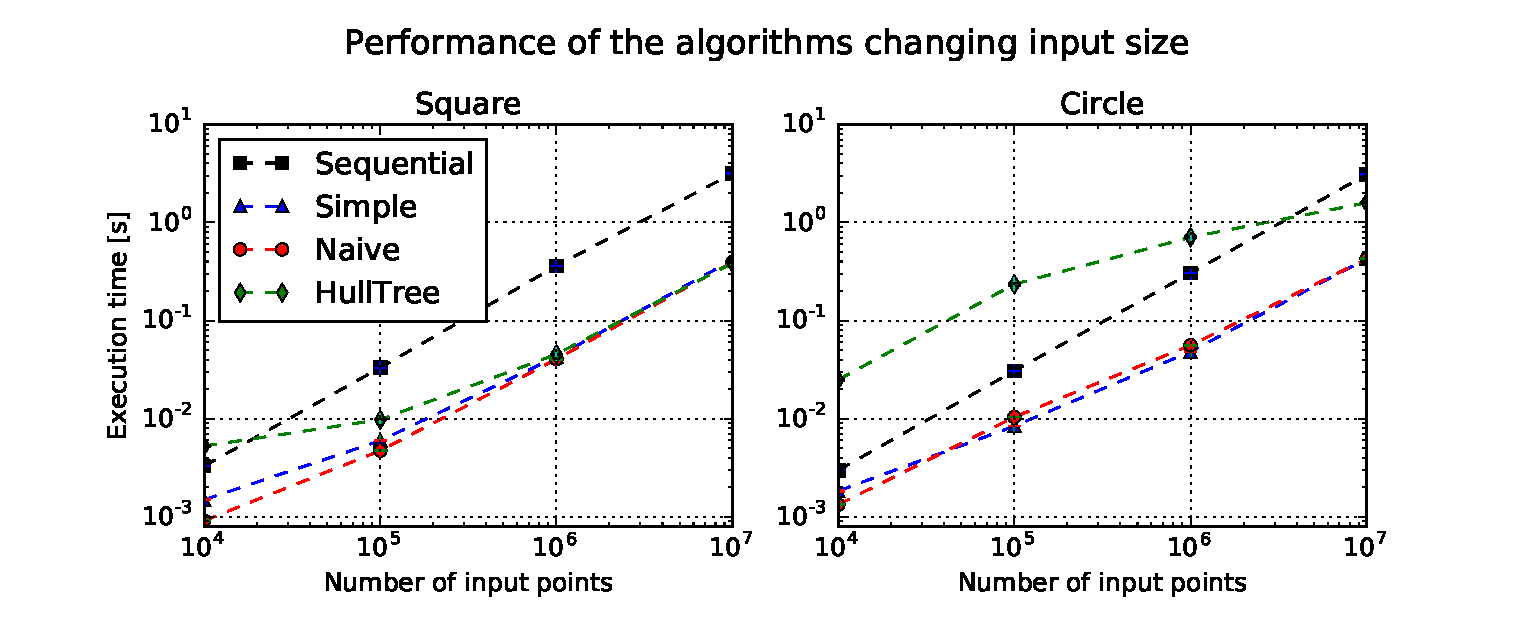
\includegraphics[scale=0.33]{./plots/time_points.eps}
  \caption{Comparison of the execution times three algorithms for 8 threads and the sequential version changing input size for square and circle\label{Input size time}}
\end{figure}

For the sequential versions the growth in execution time when increasing the number of input points is linear for all the selected shapes.
Concerning the parallel algorithms they have similar trends except for \textit{HullTree}, that performs significantly worse for small input sets [Plot \ref{Input size time}], expecially with the circle: \textit{HullTree}'s performance is even worse than the sequential one.
This is due to the creation of the data structure that for a high number of resulting points (recall that for circle almost every generated point is part of the final convex hull) needs a lot of time.

\begin{figure}[!ht]\centering
  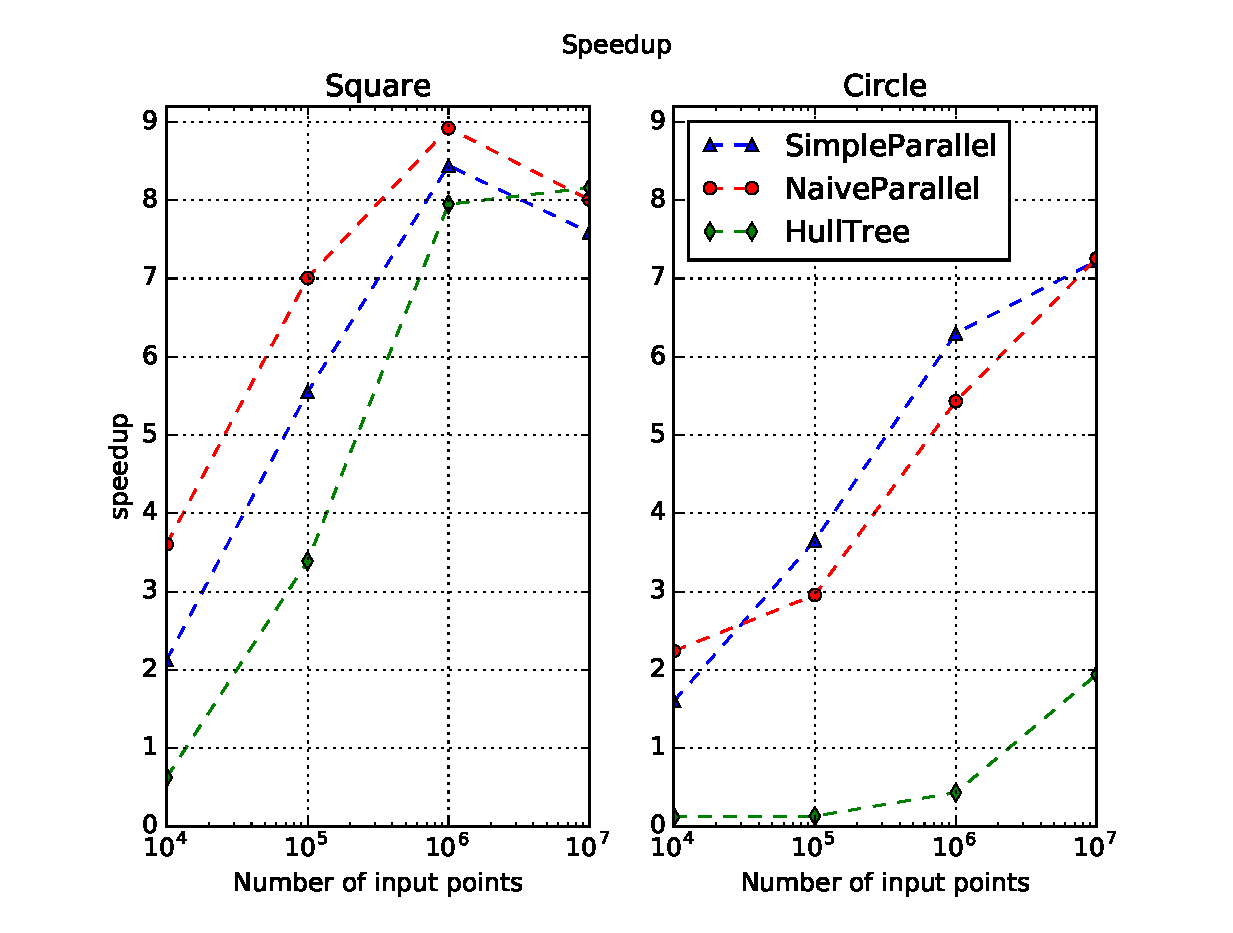
\includegraphics[scale=0.33]{./plots/speedup_points.eps}
  \caption{Speedup comparison of the three algorithms for 8 threads changing input size for square and circle\label{Input size speedup}}
\end{figure}

Looking at the speedup plots [Plot \ref{Input size speedup}] the general trend is a general growth in efficiency when increasing the size of the input set for the two shapes.

We notice a superlinear speedup around 10$^6$ points (around 9 for \textit{Naive} and 8.5 for \textit{Simple}) and 10$^7$ points (slightly above 8 for both \textit{Simple} and \textit{HullTree}.
We obtained superlinear speedup thanks to caching: splitting the input set into smaller subsets assigned to processors makes the subset fit better into cache, allowing faster accesses to the points.

\subsubsection{Change number of threads for fixed input}

Here we analyze the performance of our algorithms with the different number of processing threads under a fixed input size of 10$^6$ and 10$^7$ points.

\begin{figure}[!ht]\centering
  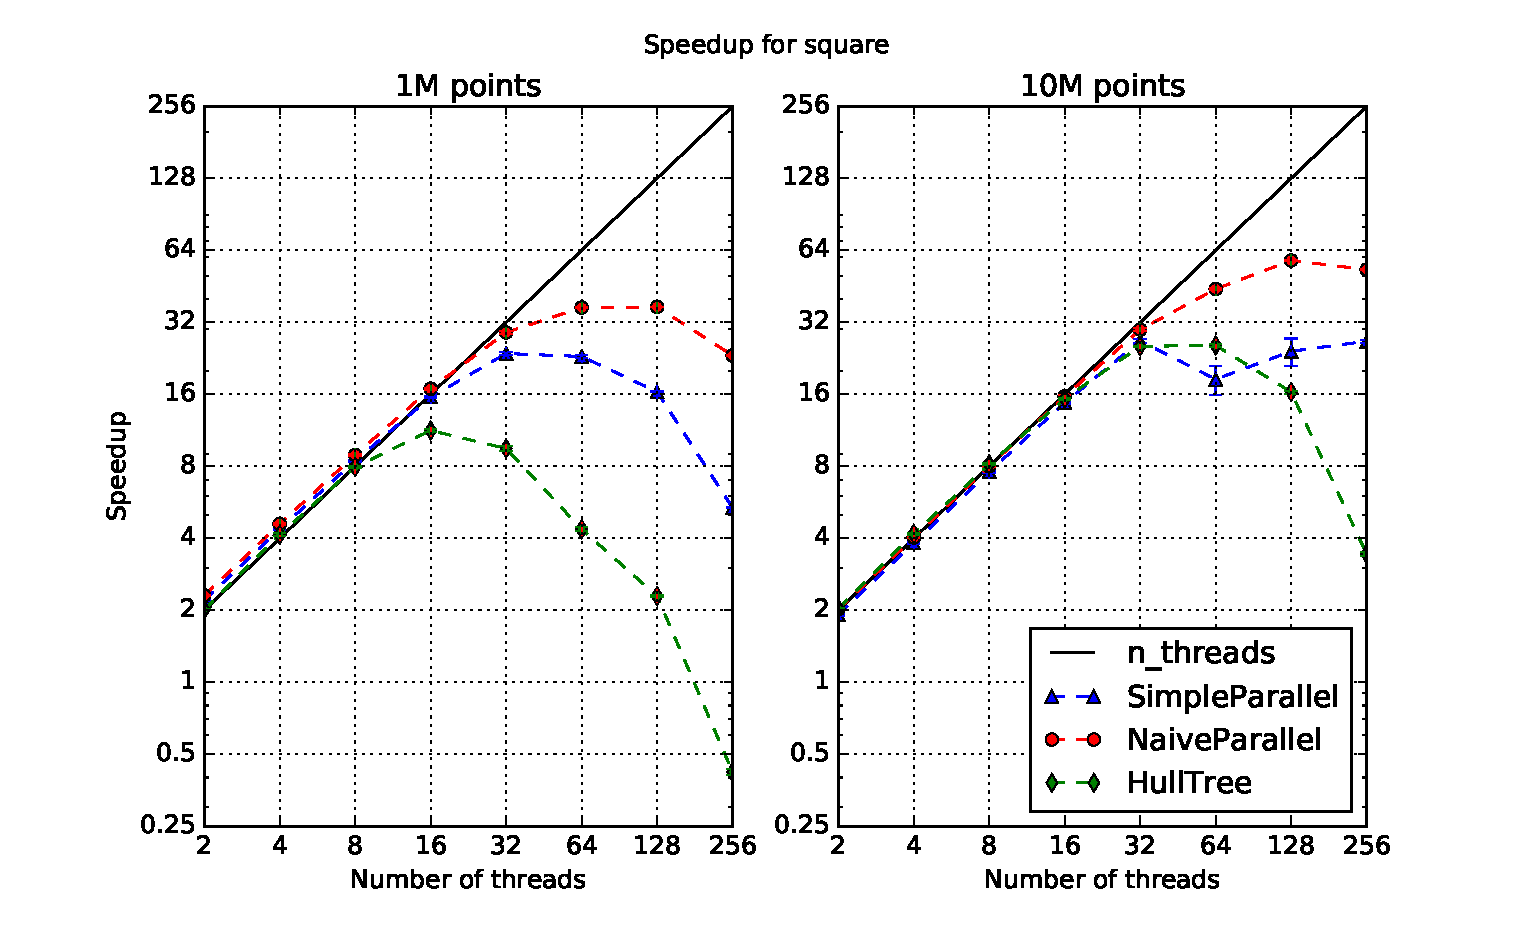
\includegraphics[scale=0.33]{./plots/speedup_xeon_square_fixed_points.eps}
  \caption{Speedup of the algorithms with the given number of threads with a square for 10$^6$ [Sequential execution time: 0.3s] and 10$^7$ [sequential execution time: 3s] points\label{Threads speedup square}}
\end{figure}

For square and disk we notice similar trends [Plot \ref{Threads speedup square}] speedup close to linear or even superlinear until around 16 threads for 10$^6$ points and 32 for 10$^7$ points then a general decrease in efficiency growth up to a point where our algorithms stop scaling and the speedup starts decreasing.

We can notice that that point is shifted to a higher number of threads when the input set is bigger. Clearly the lower the number of points the lesser the efficiency obtained by splitting the point set among threads.
After that point, the overhead added by parallelism overweights the benefits introduced by having more processing units.

This overhead is related both to the OS, that has to create, allocate and manage a high number of threads, and to the algorithms themselves:
in fact for a high number of threads, while the first part of the algorithms (separately compute convex hull on split point sets) becomes very fast, the merging itself takes more time and the two processes start becoming unbalanced.

\begin{figure}[!ht]\centering
  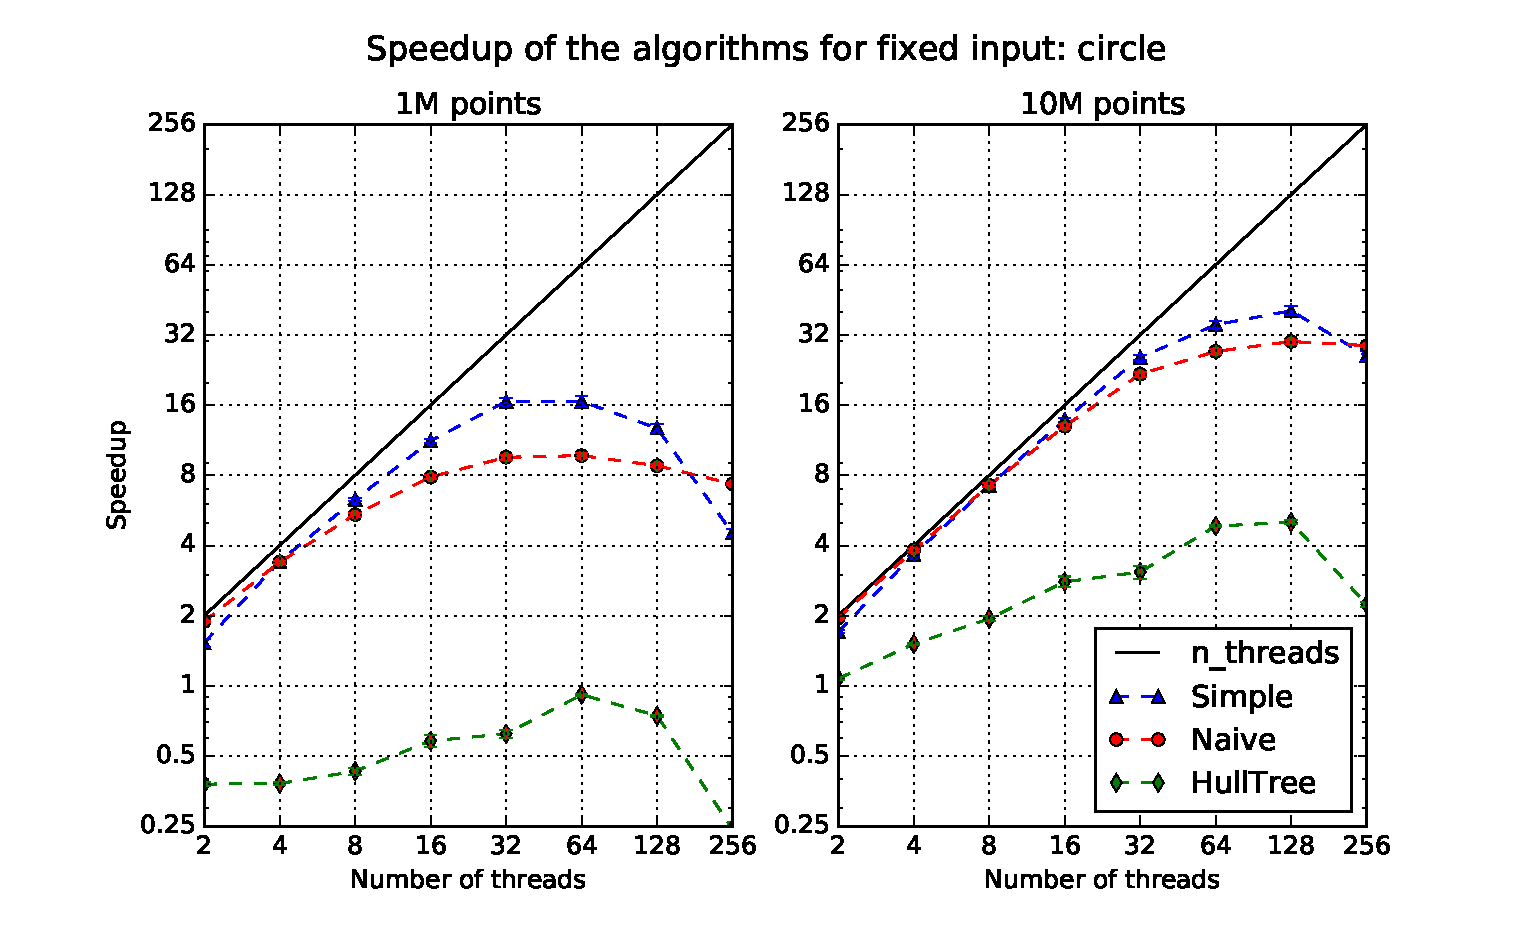
\includegraphics[scale=0.33]{./plots/speedup_xeon_circle_fixed_points.eps}
  \caption{Speedup of the algorithms with the given number of threads with a circle for 10$^6$ [sequential execution time: 0.3s] and 10$^7$ [sequential execution time: 3s] points\label{Threads speedup circle}}
\end{figure}

For circle [Plot \ref{Threads speedup circle}] the situation is again more complicated, since the HullTree algorithm has a very bad performance, but the trend is very simlar with a fast increase in efficiency followed by a close-to-steady state and a decrease in efficiency for a high number of threads.
Quantitatively the overall efficiency of the parallel algorithms is lower than the one obtained with the square and that's probably because the more memory accesses needed and the parallel overhead make the algorithms behave worse.

\subsubsection{Behavior with unoptimal number of threads}

For a number of threads that is not a power of 2, because of their implementations, Naive and HullTree algorithm behave like the closest lower power of two (i.e. with 35 threads they behave like they had 32).

\textit{Simple} algorithm, instead, is not correlated to powers of two and the performance for any number of threads is ?????????????????????????????.

\begin{figure}[!ht]\centering
  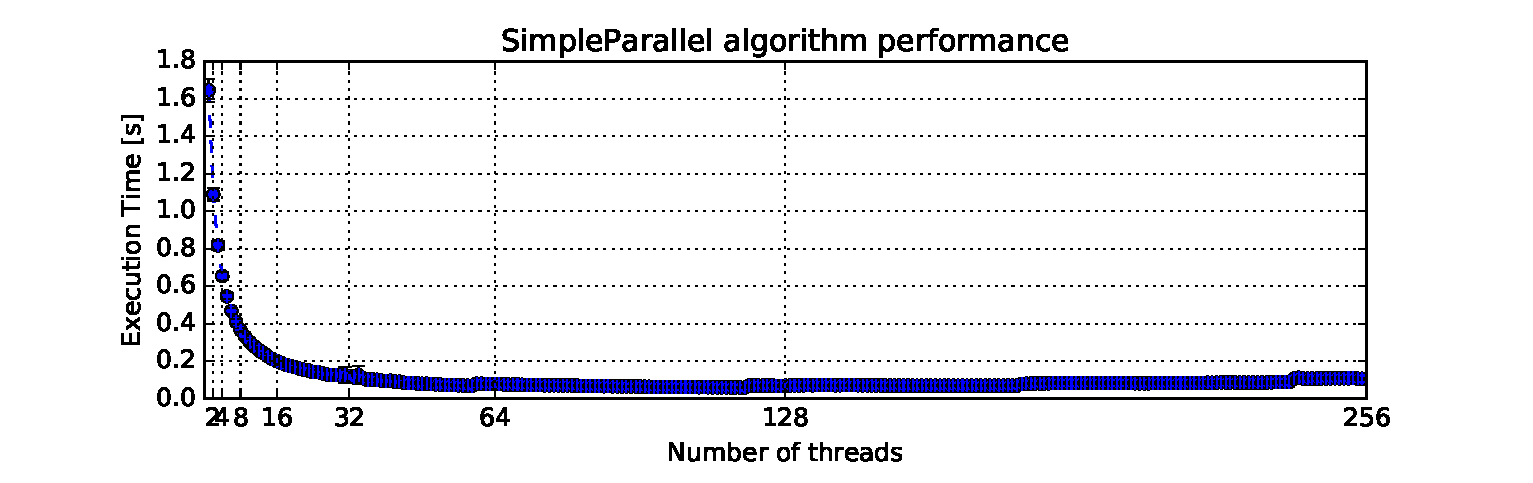
\includegraphics[scale=0.33]{./plots/total.eps}
  \caption{Execution time of Simple algorithm for a square of 10$^7$ points\label{SimpleParallel Total}}
\end{figure}


\section{Conclusions}

Here you need to summarize what you did and why this is
important. {\em Do not take the abstract} and put it in the past
tense. Remember, now the reader has (hopefully) read the report, so it
is a very different situation from the abstract. Try to highlight
important results and say the things you really want to get across
such as high-level statements (e.g., we believe that .... is the right
approach to .... Even though we only considered x, the
.... technique should be applicable ....) You can also formulate next
steps if you want. Be brief. After the conclusions there are only the references.

\section{Further comments}

Here we provide some further tips.

\mypar{Further general guidelines}

\begin{itemize}
\item For short papers, to save space, I use paragraph titles instead of
subsections, as shown in the introduction.

\item It is generally a good idea to break sections into such smaller
units for readability and since it helps you to (visually) structure the story.

\item The above section titles should be adapted to more precisely
reflect what you do.

\item Each section should be started with a very
short summary of what the reader can expect in this section. Nothing
more awkward as when the story starts and one does not know what the
direction is or the goal.

\item Make sure you define every acronym you use, no matter how
convinced you are the reader knows it.

\item Always spell-check before you submit (to us in this case).

\item Be picky. When writing a paper you should always strive for very
high quality. Many people may read it and the quality makes a big difference.
In this class, the quality is part of the grade.

\item Books helping you to write better: \cite{Higham:98} and \cite{Strunk:00}.

\item Conversion to pdf (latex users only): 

dvips -o conference.ps -t letter -Ppdf -G0 conference.dvi

and then

ps2pdf conference.ps
\end{itemize}

\mypar{Graphics} For plots that are not images {\em never} generate the bitmap formats
jpeg, gif, bmp, tif. Use eps, which means encapsulate postscript. It is
scalable since it is a vector graphic description of your graph. E.g.,
from Matlab, you can export to eps.

The format pdf is also fine for plots (you need pdflatex then), but only if the plot was never before in the format 
jpeg, gif, bmp, tif.


% References should be produced using the bibtex program from suitable
% BiBTeX files (here: bibl_conf). The IEEEbib.bst bibliography
% style file from IEEE produces unsorted bibliography list.
% -------------------------------------------------------------------------
\bibliographystyle{IEEEbib}
\bibliography{bibl_conf}

\end{document}

